% \iffalse
\let\negmedspace\undefined
\let\negthickspace\undefined
\documentclass[journal,12pt,twocolumn]{IEEEtran}
\usepackage{cite}
\usepackage{amsmath,amssymb,amsfonts,amsthm}
\usepackage{algorithmic}
\usepackage{graphicx}
\usepackage{textcomp}
\usepackage{xcolor}
\usepackage{txfonts}
\usepackage{listings}
\usepackage{enumitem}
\usepackage{mathtools}
\usepackage{gensymb}
\usepackage{comment}
\usepackage[breaklinks=true]{hyperref}
\usepackage{tkz-euclide} 
\usepackage{listings}
\usepackage{gvv}                                        
\def\inputGnumericTable{}                                 
\usepackage[latin1]{inputenc}                                
\usepackage{color}                                            
\usepackage{array}                                            
\usepackage{longtable}                                       
\usepackage{calc}                                             
\usepackage{multirow}                                         
\usepackage{hhline}                                           
\usepackage{ifthen}                                           
\usepackage{lscape}

\newtheorem{theorem}{Theorem}[section]
\newtheorem{problem}{Problem}
\newtheorem{proposition}{Proposition}[section]
\newtheorem{lemma}{Lemma}[section]
\newtheorem{corollary}[theorem]{Corollary}
\newtheorem{example}{Example}[section]
\newtheorem{definition}[problem]{Definition}
\newcommand{\BEQA}{\begin{eqnarray}}
\newcommand{\EEQA}{\end{eqnarray}}
\newcommand{\define}{\stackrel{\triangle}{=}}
\theoremstyle{remark}
\newtheorem{rem}{Remark}

\begin{document}

\bibliographystyle{IEEEtran}
\vspace{3cm}

\title{NCERT 11.9.2.3}
\author{EE23BTECH11043 - BHUVANESH SUNIL NEHETE$^{*}$% <-this % stops a space
}
\maketitle
\newpage
\bigskip

\renewcommand{\thefigure}{\theenumi}
\renewcommand{\thetable}{\theenumi}

\bibliographystyle{IEEEtran}

\textbf{Question:}

In an A.P. the first term is 2 and the sum of the first five terms is one-fourth of the next five terms. Show that 20\textsuperscript{th} term is $-112$.

\solution
\begin{table}[h]
\renewcommand\thetable{1}
    \centering
    \begin{tabular}{|c|c|c|}
        \hline
        \textbf{Parameter} & \textbf{Description} & \textbf{Value}\\
        \hline
        $x(0)$ & First term & $2$\\
        \hline
        $x(19)$ & $20\textsuperscript{th}$ term & $-112$\\
        \hline
        $y(n)$ & sum upto $n\textsuperscript{th}$ term & \\
        \hline
    \end{tabular}
    \caption{Input data}
  \label{input data}
\end{table}


General term can be written as
\begin{align}
    x\brak{n} = \brak{x\brak{0} + nd}u\brak{n}
\end{align}
y\brak{n} is the sum upto n terms,
    \begin{align}
        y\brak{n} &= x\brak{0}\brak{n+1} + \frac{n\brak{n+1}}{2}d
    \end{align}
Given, 
   \begin{align}
       \sum_{n=0}^{4}x\brak{n} = \frac{1}{4}\sum_{n=5}^{9}x\brak{n}
   \end{align}
Simplifying:
    \begin{align}
        y\brak{4} &= \frac{1}{4}\brak{y\brak{9}-y\brak{4}}\\
        \implies 5x\brak{0} + 10d &= \frac{1}{4}\brak{5x\brak{0} + 35d}\\
        x\brak{0} &= \frac{-d}{3}\\
        \implies d &= -6 \label{eq1}
    \end{align}
From \eqref{eq1} and \tabref{input data}
    \begin{align}
        x\brak{19}&=x\brak{0}+19d\\ 
        &= -112
   \end{align} 
From \eqref{eq1} and \tabref{input data}:
    \begin{align}
        \implies x\brak{n}&=\brak{2-6n}u\brak{n} \label{eq3}
    \end{align}    
From \eqref{eq3} :
    \begin{align}
        X\brak{z}=\frac{2}{1-z^{-1}} - \frac{6z^{-1}}{\brak{1-z^{-1}}^{2}} \quad |z|>1
    \end{align}

    \begin{figure}[ht]
    \renewcommand\thefigure{1}
        \centering
        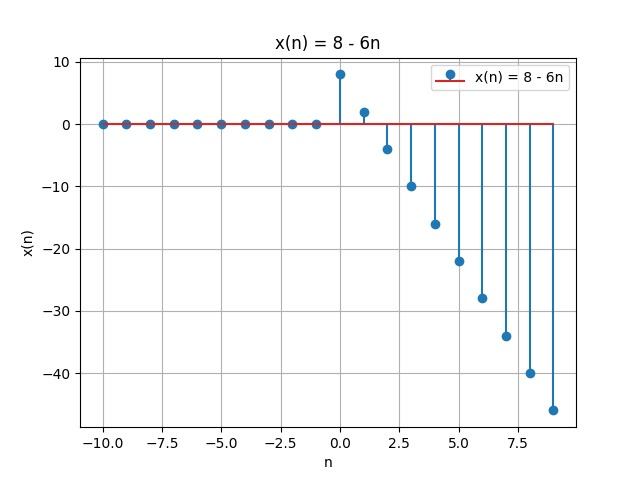
\includegraphics[width=1\linewidth]{figs/Figure_1.png}
        \caption{graph of x\brak{n} = 2 - 6n}
    \end{figure}

\end{document}
